\section{Neutrinos Today}\label{ch:nu_today}
%%%%%%%%%%%%%%%%%%%%%%%%%%%%%%%%%%%%%%%%%%%%%%
Experimental detection of the cosmic background neutrinos is a challenge of great interest \cite{Stodolsky:1974aq,Cabibbo:1982bb,Shvartsman,Langacker:1982ih,Smith:1983jj,Ferreras:1995wf,Hagmann:1999kf,Duda:2001hd,Gelmini:2004hg,Ringwald:2009bg,Liao:2012wb,Hedman:2013hha}. With the  recently proposed PTOLEMY experiment, which aims to detect relic  electron-neutrino capture by tritium \cite{Betts:2013uya}, the characterization of the relic neutrino background is increasingly relevant.  Using our  characterization of the neutrino distribution after freeze-out and the subsequent free-streaming dynamics from Section  \ref{ch:model_ind} and \cite{Birrell:2012gg}, we lay groundwork for a characterization of the present day relic neutrino spectrum, which we explore  from the  perspective of an observer moving relative to the neutrino background, including the dependence on neutrino mass and effecitve number of neuntrinos, $N_\nu^{\mathrm{eff}}$. Beyond consideration of the observable neutrino distributions, we evaluate the ${\cal O}(G_F^2)$ mechanical drag force acting on the moving observer. This section is adapted from the work in \cite{Birrell:2014qna}.




%%%%%%%%%%%%%%%%%
\subsection{Neutrino Distribution in a Moving Frame}

The neutrino background and the cosmic microwave background (CMB) were in equilibrium until decoupling (called freeze-out) at $T_k\simeq {\cal O}{\rm (MeV)}$, hence one surmises that an observer would have the same relative velocity relative to the relic neutrino background  as with CMB. As a particular example in considering the spectrum, we present in more detail the case of an observer comoving with  Earth velocity $v_\oplus=300$\,km/s relative to the CMB,  modulated by orbital velocity ($\pm29.8$\,km/s).  We will write velocities in units of $c$, though our specific results will be presented in km/s.

In the cosmological setting, for $T<T_k$ the neutrino spectrum evolves according to the well known Fermi-Dirac-Einstein-Vlasov (FDEV) free-streaming  distribution~\cite{Langacker:1982ih,Choquet-Bruhat:2009xil,Wong:2011ip,Birrell:2012gg}.  By casting it in a relativistically invariant form we can then make a transformation to the rest frame of an observer moving with relative velocity $v_{\text{rel}}$ and obtain
\begin{align}\label{neutrino_dist_B}
f(p^\mu)=&\frac{1}{\Upsilon^{-1} e^{\sqrt{(p^\mu U_\mu)^2-m_\nu^2}/T_\nu}+1}\,.
\end{align}
The 4-vector characterizing the rest frame of the neutrino FDEV distribution is
\begin{equation}\label{4_vel}
U^\mu=(\gamma,0,0,v_{\text{rel}}\gamma)\,,\hspace{2mm} \gamma={1}/{\sqrt{1-v_{\text{rel}}^2}}\,,
\end{equation} 
where we have chosen coordinates so that the relative motion is in the $z$-direction. The neutrino effective temperature $T_\nu(t)= T_k\,(a(t_k)/a(t))$ is the scale-shifted freeze-out temperature $T_k$. Here $a(t)$ is the cosmological scale factor where $\dot a(t)/a(t)\equiv H$ is the observable Hubble parameter. $\Upsilon$ is the  fugacity factor, here describing the underpopulation of neutrino phase space that was frozen into the neutrino FDEV distribution in the process of decoupling from the $e^\pm,\gamma$-QED background  plasma.

There are several available bounds on neutrino masses. Neutrino energy and pressure components are important before photon freeze-out and thus $m_\nu$ impacts Universe dynamics. The analysis of CMB data alone leads to $\sum_i m_\nu^i<0.66$eV ($i=e,\mu,\tau$) and including Baryon Acoustic Oscillation (BAO) gives $\sum m_\nu<0.23$eV~\cite{Planck:2013pxb}.  {\small PLANCK CMB} with lensing observations~\cite{Battye:2013xqa} lead to  $\sum m_{\nu}=0.32\pm0.081$ eV. Upper bounds have been placed on the electron neutrino mass in direct laboratory measurements  $m_{\bar\nu_e}<2.05$eV~\cite{Troitsk:2011cvm}.   In the subsequent analysis we will focus on the neutrino mass range $0.05$eV to $2$eV in order to show that direct measurement sensitivity allows the exploration of a wide mass range. 



 The relations in Section \ref{Tnugam}, see also~\cite{Birrell:2012gg}, determine $T_\nu/T_\gamma$ and  $\Upsilon$ in terms of the measured  value of  $N_\nu^{\mathrm{eff}}$ under the assumption of a strictly SM-particle inventory.  In the following we treat $N_\nu^{\mathrm{eff}}$  as a variable model parameter and use the above mentioned relations to characterize our results in terms of $N_\nu^{\mathrm{eff}}$.


\subsection{Velocity, Energy, and Wavelength Distributions}

Using \req{neutrino_dist_B}, the normalized FDEV velocity distribution for an observer in relative motion has the form
\begin{align} \label{fvdistrib}
&f_v=\frac{g_\nu}{n_\nu 4\pi^2}\!\!\!\int_0^\pi \!\!\!\!\frac{ p^2dp/dv\sin(\phi) d\phi}{\Upsilon^{-1}e^{\sqrt{( E-v_{\text{rel}} p \cos(\phi))^2\gamma^2-m_\nu^2}/T_\nu}+1}\,,\notag\\
&p(v)=\frac{m_\nu v}{\sqrt{1-v^2}}\,,\qquad \frac{dp}{dv}=\frac{m_\nu}{(1-v^2)^{3/2}}\,.
\end{align}
The normalization $n_\nu$ depends on $N_\nu^{\mathrm{eff}}$ but not on $m_\nu$ since decoupling occurred at $T_k\gg m_\nu$. For each neutrino flavor (all flavors are equilibrated by oscillations) we have, per neutrino or antineutrino and at non-relativistic relative velocity,
\begin{equation}\label{nnu}
n_\nu=[-0.3517(\delta N_\nu^{\mathrm{eff}})^2+6.717\delta N_\nu^{\mathrm{eff}}+56.06]\,{\rm cm}^{-3}
\end{equation}
($\delta N_\nu^{\mathrm{eff}}\equiv N_\nu^{\mathrm{eff}}-3$), compare to Eq.(55) in Ref.~\cite{Birrell:2012gg}.

We show $f_v$ in Figure \ref{fig:rel_v_dist_300}   for several values of the neutrino mass, $v_{\text{rel}}=300$ km/s, and $N_\nu^{\mathrm{eff}}=3.046$ (solid lines) and $N_\nu^{\mathrm{eff}}=3.62$ (dashed lines). As expected, the lighter the neutrino, the more $f_v$  is weighted towards higher velocities with the velocity becoming visibly peaked about $v_{\text{rel}}$ for $m_\nu=2$ eV. 
%%%%%%%%%%%%%%%%%%%%%%%%%%%%%%%%%%%%%%%
%%%%%%%%%%%%%%%%%%%%%%%%%%%%%%%%%%%%%%%
\begin{figure}%[h]
\centerline{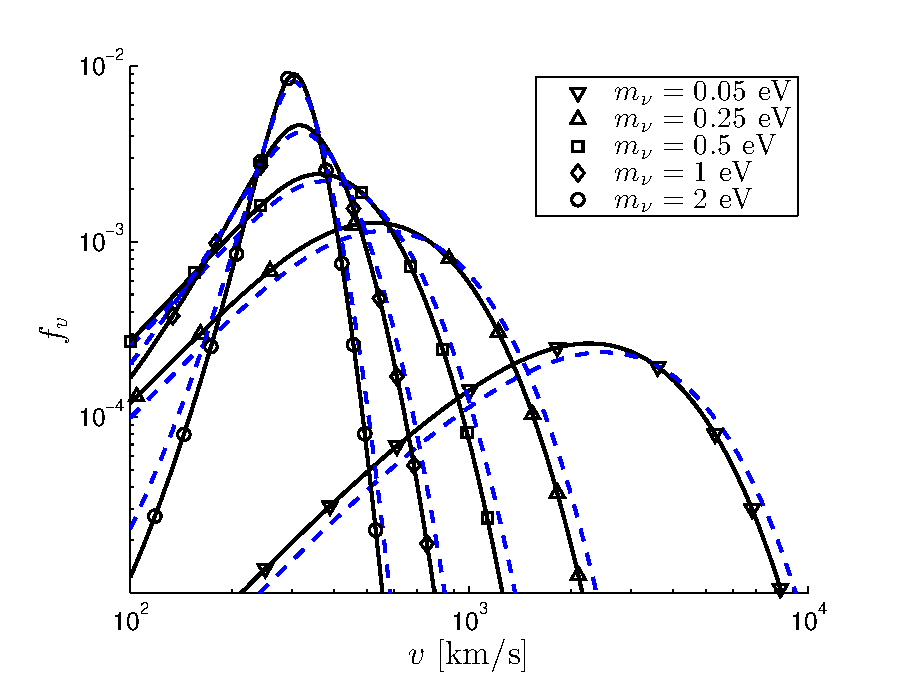
\includegraphics[height=6cm]{04-birrell/NeutrinoDistributionToday/Figures/rel_v_dist_300.eps}}
\caption{\cccite{Birrell:2014qna}. Normalized neutrino FDEV velocity distribution in the Earth frame. We show the distribution for $N_\nu^{\mathrm{eff}}=3.046$ (solid lines) and $N_\nu^{\mathrm{eff}}=3.62$ (dashed lines).}\label{fig:rel_v_dist_300}
 \end{figure}
%%%%%%%%%%%%%%%%%%%%%%%%%%%%%%%%%%%%%%%

A similar procedure produces the normalized FDEV energy distribution $f_E$.  In \req{fvdistrib} we replace $dp/dv\to dp/dE$ where it is understood that 
\begin{equation}
p(E)=\sqrt{E^2-m_\nu^2},\qquad \frac{dp}{dE}=\frac{E}{p}.
\end{equation}
We show $f_E$ in Figure \ref{fig:E_dist_300}  for several values of the neutrino mass, $v_{\text{rel}}=300$ km/s, and $N_\nu^{\mathrm{eff}}=3.046$ (solid lines) and $N_\nu^{\mathrm{eff}}=3.62$ (dashed lines). The width of the FDEV energy distribution is on the micro-eV scale and the kinetic energy $T=E-m_\nu$ is peaked about $T=\frac{1}{2}m_\nu v_{\text{rel}}^2$, implying that the relative velocity between the Earth and the CMB is the dominant factor for $m_\nu>0.1$ eV.
%%%%%%%%%%%%%%%%%%%%%%%%%%%%%%%%%%%%%%%
\begin{figure}%[h]
\centerline{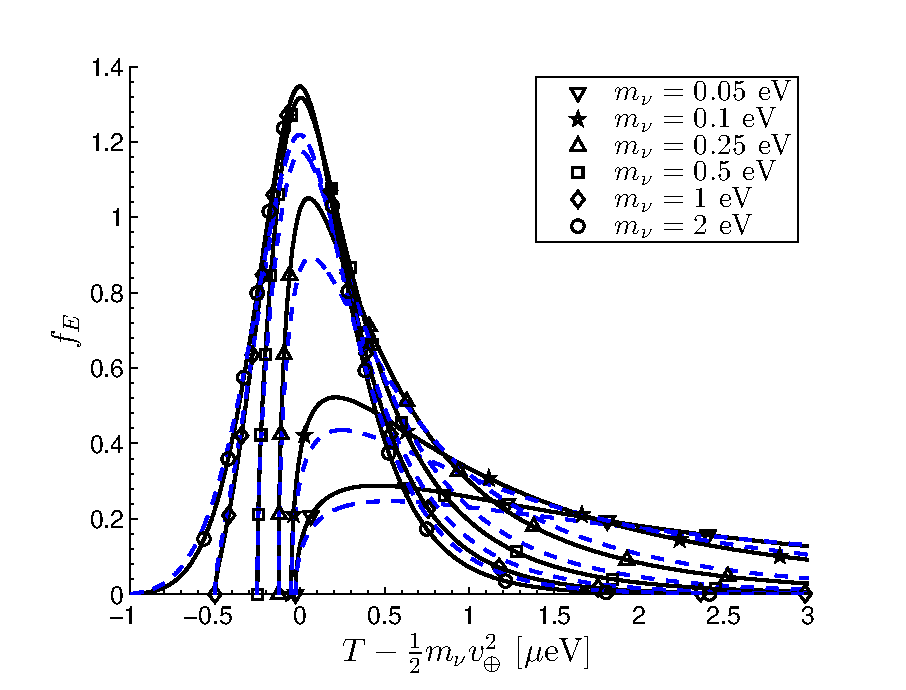
\includegraphics[height=6cm]{04-birrell/NeutrinoDistributionToday/Figures/E_dist_300.eps}}
\caption{\cccite{Birrell:2014qna}. Neutrino FDEV energy distribution in the Earth frame. We show the distribution for $N_\nu=3.046$ (solid lines) and $N_\nu=3.62$ (dashed lines). }\label{fig:E_dist_300}
 \end{figure}
%%%%%%%%%%%%%%%%%%%%%%%%%%%%%%%%%%%%%%%


By multiplying $f_E$ by the neutrino velocity and number density for a single neutrino flavor (without anti-neutrinos) we obtain the particle flux density,
 \begin{equation}
 \frac{dJ}{dE}\equiv\frac{dn}{dAdtdE}\,,
\end{equation} 
shown in Figure \ref{fig:flux_dist}. We show the result for $N_\nu^{\mathrm{eff}}=3.046$ (solid lines) and $N_\nu^{\mathrm{eff}}=3.62$ (dashed lines). The flux is normalized in these cases to a local denisty $56.36$~cm${}^{-3}$ and $60.10$~cm${}^{-3}$ respectively. The precise neutrino flux in the Earth frame is significant for efforts to detect relic neutrinos, such as the PTOLEMY experiment~\cite{Betts:2013uya}. The energy dependence of the flux shows a large sensitivity to the mass. However, the maximal fluxes do not vary significantly with $m$. In fact the maximum values are independent of $m$ when $v_{\text{rel}}=0$, as follows from the fact that $v=p/E=dE/dp$.  In the Earth frame, where $0<v_\oplus\ll c$, this translates into only a small variation in the maximal flux.
%%%%%%%%%%%%%%%%%%%%%%%%%%%%%%%%%%%%%%%
\begin{figure}%[h]
\centerline{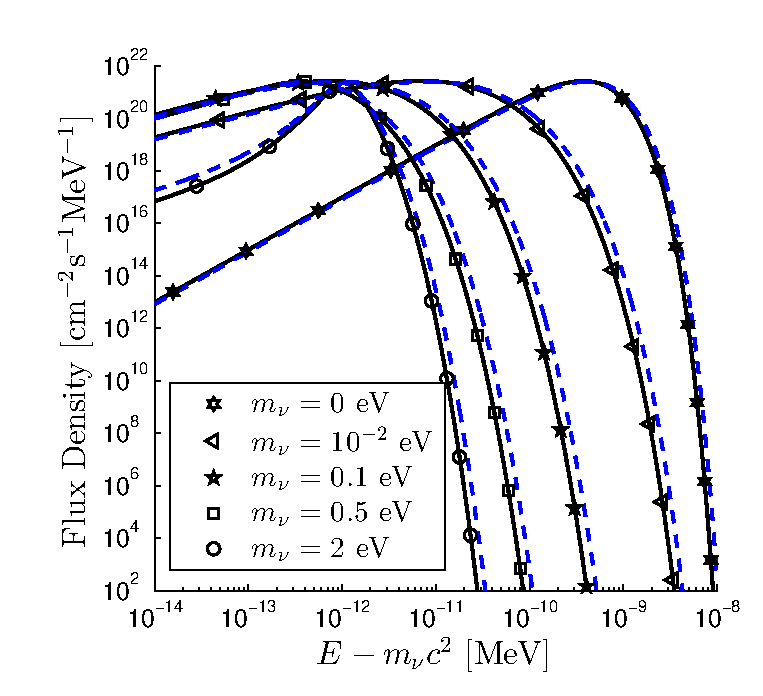
\includegraphics[height=7cm]{04-birrell/NeutrinoDistributionToday/Figures/flux_dist.eps}}
\caption{\cccite{Birrell:2014qna}.  Neutrino flux density in the Earth frame. We show the result for $N_\nu^{\mathrm{eff}}=3.046$ (solid lines) and $N_\nu^{\mathrm{eff}}=3.62$ (dashed lines) for an observer moving with $v_\oplus=300$\,km/s.}\label{fig:flux_dist}
 \end{figure}
%%%%%%%%%%%%%%%%%%%%%%%%%%%%%%%%%%%%%%%

Using $\lambda=2\pi/p$ we find  the normalized FDEV de Broglie wavelength distribution
\begin{equation}
%\frac{dn}{d\lambda}
f_\lambda=\frac{ 2\pi g_\nu}{n_\nu\lambda^4}\!\!\int_0^\pi\!\!\! \!\frac{\sin(\phi) d\phi}{\Upsilon^{-1}e^{\sqrt{( E-v_{\text{rel}} p \cos(\phi))^2\gamma^2-m_\nu^2}/T_\nu}\!\!+\!1}\,,
\end{equation}
shown in Figure \ref{fig:deBrogle_300} for $v_{\text{rel}}=300$ km/s and for several values $m_\nu$ comparing  $N_\nu^{\mathrm{eff}}=3.046$ with $N_\nu^{\mathrm{eff}}=3.62$. %  While the FDEV distributions are peaked at the millimeter wavelength scale, to discriminate dependence on neutrino masses it is necessary to consider somewhat larger wavelengths. 
%%%%%%%%%%%%%%%%%%%%%%%%%%%%%%%%%%%%%%%
\begin{figure}%[h]
\begin{minipage}{\linewidth}
\makebox[0.5\linewidth]%
{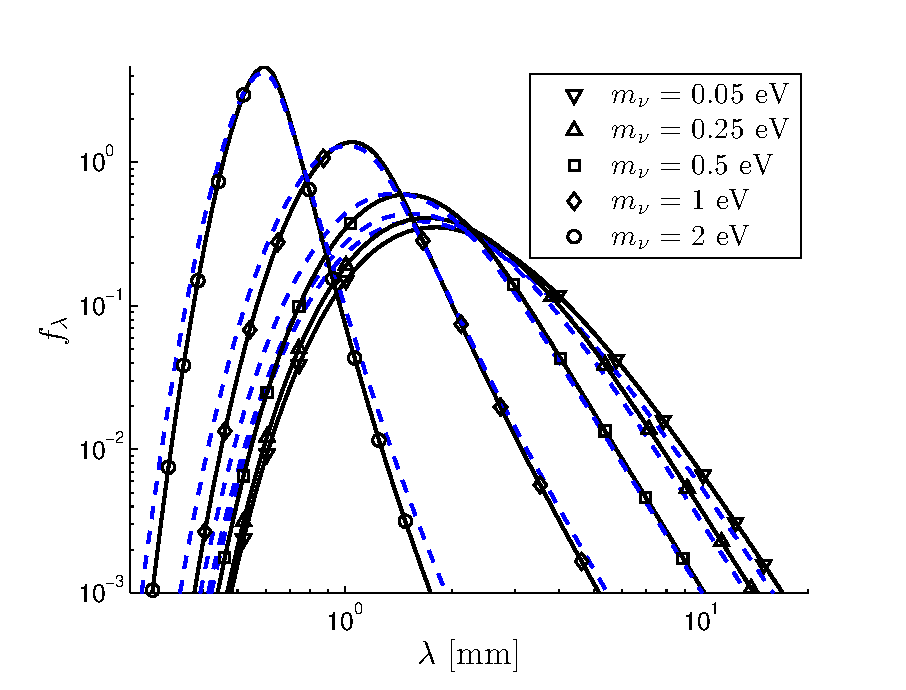
\includegraphics[height=5.8cm]{04-birrell/NeutrinoDistributionToday/Figures/deBrogle_300.eps}}
\makebox[0.5\linewidth]%
{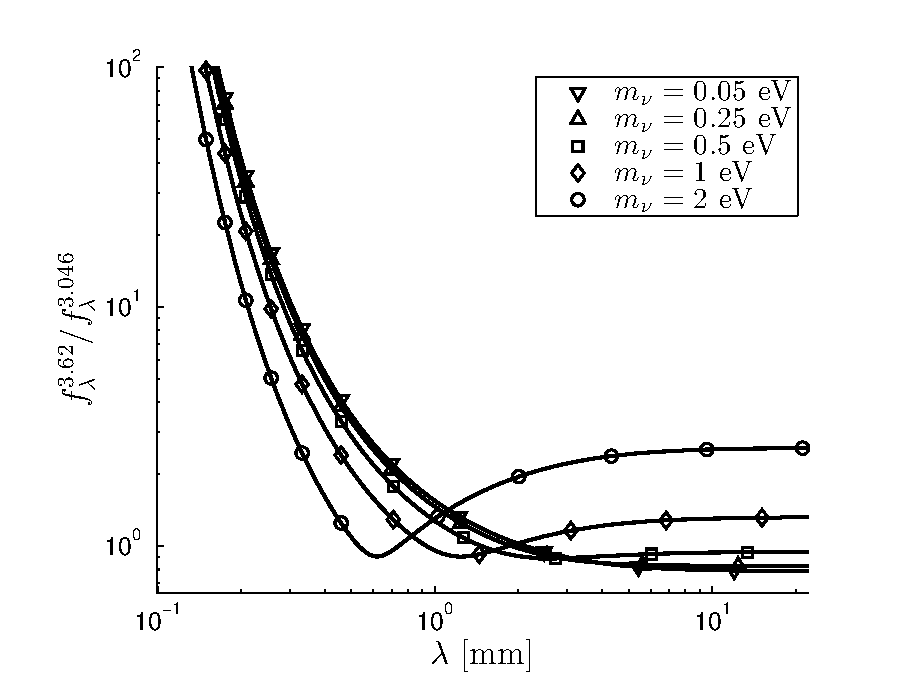
\includegraphics[height=5.8cm]{04-birrell/NeutrinoDistributionToday/Figures/f_ratio.eps}}
\end{minipage}
\caption{\cccite{Birrell:2014qna}.  Neutrino  FDEV de Broglie wavelength  distribution in the Earth frame. We show in top panel the distribution for $N_\nu^{\mathrm{eff}}=3.046$ (solid lines) and $N_\nu^{\mathrm{eff}}=3.62$ (dashed lines) and in bottom panel their ratio.}\label{fig:deBrogle_300}
 \end{figure}
%%%%%%%%%%%%%%%%%%%%%%%%%%%%%%%%%%%%%%%%%%%%%%%%%

\subsection{Drag Force}
Given the neutrino distribution, we evaluate the drag force due to the anisotropy of the neutrino distribution in the rest frame of the moving object for $N_\nu^{\mathrm{eff}}=3.046$. The relic neutrinos will undergo potential scattering with the scale of the potential strength being
\begin{equation}\label{V0}
V_0=CG_F\rho_{N_c},\hspace{2mm} \rho_N\equiv N_c/R^3
\end{equation}
where $R$ is the linear size of the detector.  When the detector size is smaller than the quantum de Broglie wavelength of the neutrino, all scattering centers are added coherently to for the target effective `charge' $N_c$.  $\rho_{N_c}$ is the charge density, and C=O(1) and is depending on material composition of the object. Such considerations are of interest both for scattering from terrestrial detectors, as well as for ultra-dense objects of neutron star matter density, e.g.   strangelet  CUDOS~\cite{Rafelski:2011bby} - recall that such nuclear matter fragments with $R<\lambda$  despite their small size would have a mass rivaling that of large meteors. We find $V_0\simeq 10^{-13}$ eV for normal matter densities, but for nuclear target density a potential well with $V_0\simeq {\cal O}(10 {\rm eV})$.  

We consider relic neutrino potential scattering to obtain the average momentum transfer to the target and hence the drag force. The particle flux per unit volume in momentum space is
\begin{equation}\label{dn_quantum}
\frac{dn}{dtd Ad^3{\bf p}}({\bf p})=\frac{2}{(2\pi)^3}f({\bf p})p/m_\nu\,,\hspace{2mm} p\equiv |{\bf p}|\,,
\end{equation}
where the factor of two comes from combining neutrinos and anti-neutrinos of a given flavor. Our use of non-relativistic velocity is justified by Figure \ref{fig:rel_v_dist_300}.  The recoil change in detector momentum per unit time is  
\begin{align}
\frac{d{\bf p}}{dt}=& \int  {\bf q}A \frac{dn}{dtdAd^3p}({\bf p})d^3p\,,\\
{\bf q}A\equiv &\int ({\bf p}-{\bf p_f})\frac{d\sigma}{ d\Omega}({\bf p_f},{\bf p})d\Omega\,.
\end{align}
Here ${\bf p}$ and ${\bf p}_f$, the incoming and outgoing momenta respectively, have the same magnitude. $qA$ is the momentum transfer times area, averaged over outgoing momenta, and $d\Omega$ is the solid angle for to ${\bf p}_f$.  

For a spherically symmetric potential the differential cross section depends only on the incoming energy and the angle $\phi$ between ${\bf p}$ and ${\bf p_f}$.  Therefore, for each ${\bf p}$ the integral over $d\Omega$ of the components orthogonal to ${\bf p}$ is zero by symmetry.  This implies
\begin{align}
{\bf q}A\equiv &2\pi{\bf p}\int(1-\cos(\phi))\frac{d\sigma}{ d\Omega}(p,\phi)\sin(\phi)d\phi\,.
\end{align}
The only angular dependence in the neutrino distribution is in ${\bf p}\cdot {\bf\hat z}$ and therefore the components of the force orthogonal to ${\bf \hat z}$ integrate to zero, giving
\begin{align}\label{drag}
\frac{d{\bf p}}{dt}=&\frac{{\bf\hat z}}{\pi m_\nu } \int p^4g(p) f(p,\tilde\phi) \cos(\tilde\phi) \sin(\tilde\phi) dpd\tilde\phi\,,\\
g(p)\equiv& \int_0^\pi(1-\cos(\phi))\frac{d\sigma}{ d\Omega}(p,\phi)\sin(\phi)d\phi\,.\label{geq}
\end{align}

For the case of normal density matter, the Born approximation is valid due to the weakness of the potential compared to the neutrino energy seen in Figure \ref{fig:E_dist_300}. To obtain an order of magnitude estimate, we take a Gaussian potential \begin{equation}
V(r)=V_0e^{-r^2/R^2}
\end{equation}
for which the differential cross section in the Born approximation can be analytically evaluated
\begin{align}
&\frac{d\sigma}{ d\Omega}(p,\phi)=\frac{\pi m_\nu^2V_0^2R^6}{4}e^{-q^2R^2/2}\,,\notag\\
&q=|{\bf p}-{\bf p}_f|=2p\sin(\phi/2)\,.
\end{align}
The integral over $\phi$ in \req{geq} can also be done analytically, giving
\begin{align}
g(p)=&\pi m_\nu^2V_0^2R^6\frac{1-(2R^2p^2+1)e^{-2R^2p^2}}{4R^4p^4}\,.
\end{align}
 In the long and short wavelength limit we have 
\begin{align}
\label{long_wave_drag}
&g(p)\simeq\frac{\pi}{2} m_\nu^2V_0^2R^6\,,\quad pR\ll 1\,,\\
&F_L\simeq \frac{m_\nu V_0^2R^6}{2} \int p^4 f(p,\tilde\phi) \cos(\tilde\phi) \sin(\tilde\phi) dpd\tilde\phi\,,\notag\\
\label{short_wave_drag}
&g(p)\simeq\frac{\pi m_\nu^2V_0^2R^2}{4p^4}\,, 
\quad pR\gg 1\,,\\
&F_S\simeq \frac{ m_\nu V_0^2R^2}{4} \int f(p,\tilde\phi) \cos(\tilde\phi) \sin(\tilde\phi) dpd\tilde\phi\notag\,.
\end{align}
 We also note that in the short wavelength limit, our coherent scattering treatment is only applicable to properly prepared structured targets \cite{Liao:2012wb}.

Inserting \req{V0} we see that this force is $O(G_F^2)$, see also \cite{Shvartsman,Smith:1983jj,Gelmini:2004hg}, as compared to the $O(G_F)$ effects debated in  \cite{Opher:1974drq,Lewis:1979mu,Opher2,Cabibbo:1982bb,Langacker:1982ih,Smith:1983jj,Ferreras:1995wf}. In long wavelength limit the size $R$ cancels, in favor of $N_c^2$ which explicitly shows that scattering is on the square of the charges of the target. This results in an enhancement of the force by a factor of $N_c$ over the incoherent scattering case, due to $V_0^2$ scaling with $N_c^2$. This effect exactly parallels the proposed detection of supernovae MeV energy scale neutrinos by means of collisions with the entire atomic nucleus~\cite{Divari:2012zz}.  




Fits to the integrals in the above force formulas \req{long_wave_drag} and \req{short_wave_drag} can be obtained in the region $0.005 \text{eV}\leq m_\nu\leq 0.25\text{eV}$, $v_\text{rel}\leq 300$km/s, yielding
\begin{align}\label{F_L}
F_L\!=&8\,10^{-34}{\rm N}\!\left(\!\frac{m_\nu}{0.1 \text{eV}}\!\right)^{\!\!2}\!\! \left(\!\frac{V_0}{1\text{peV}}\!\right)^{\!\!2}\!\!\left(\!\frac{R}{1\text{mm}}\!\right)^{\!\! 6} \!\!\frac{v_{\text{rel}}}{v_\oplus},\\[0.2cm]
F_S=&2\, 10^{-35}{\rm N}\!\left(\!\frac{m_\nu}{0.1\text{eV}}\!\right)^{\!\!2}\! \left(\!\frac{V_0}{1\text{peV}}\!\right)^{\!\!2}\!\!\left(\!\frac{R}{1\text{mm}}\!\right)^{\!\!2}\times\notag \\
&\hspace*{1.5cm}\times\frac{v_{\text{rel}}}{v_\oplus}\!\left(\!1\!-\!0.2\frac{m_\nu}{0.1\text{eV}}\frac{v_{\text{rel}}}{v_\oplus}\right).
\end{align}
We emphasize that they are not valid in the limit as $m_\nu\rightarrow 0$. Considering that the current frontier of precision force measurements at the level of individual ions is on the order of $10^{-24}$N \cite{Biercuk}, the ${\cal O}(G_F^2)$ force on a coherent mm-sized terrestrial detector is negligible, despite the factor of $N_c$ enhancement. 

We now consider scattering from nuclear matter density $\rho_N\simeq 3 \, 10^{8}{\rm kg/mm}^3$ objects where $V_0={\cal O}(10\text{eV})$ is effectively infinite compared to the neutrino energy unless the object velocity relative to the neutrino background is ultra-relativistic.  Therefore we are in the hard `ball' scattering limit. As with the analysis for normal matter density, we will investigate both the long and short wavelength limits. In the long wavelength limit, only the S-wave contributes to hard sphere scattering and $d\sigma/d\Omega=R^2$, independent of angle. Using \req{drag} and a similar fit to \req{F_L} gives
\begin{align}\label{FLHard}
F_L=&\frac{2\pi^2R^2}{\pi m_\nu} \int p^4 f(p,\tilde\phi) \cos(\tilde\phi) \sin(\tilde\phi) dpd\tilde\phi\notag\\
\simeq &\, 2\, 10^{-22}{\rm N}\left(\frac{R}{1\text{mm}}\right)^2\frac{v_{\text{rel}}}{v_\oplus}\,.
\end{align}
In particular the force is independent of $m_\nu$.  We also note that at high velocity, \req{FLHard}  underestimates the drag force. The resulting acceleration is
\begin{equation}
a=4\, 10^{-31}\frac{m}{s^2}\frac{v_{\text{rel}} }{v_\oplus}\! \left(\frac{R}{1\text{mm}}\right)^{-1}\!\!\left(\frac{\rho}{\rho_N}\right)^{-1}\,.\!\!
\end{equation}
The Newtonian drag time constant, $v_{\rm rel}/a$, is
\begin{equation}
\tau= 2\,10^{28}\text{yr}\frac{R}{1\text{mm}}\,\frac{\rho}{\rho_N}\,,
\end{equation}
which suggests that the compact object produced early on in stellar evolution remain largely unaltered.

The last case to consider is the short wavelength hard sphere scattering limit.  This limit is classical and so we no longer treat it as quantum mechanical potential scattering, but rather as elastic scattering of point particle neutrinos from a hard sphere of radius $R$.  For a single scattering event where the component of the momentum normal to the sphere is ${\bf p}^\perp=({\bf p}\cdot \hat {\bf r}) \hat {\bf r}$, the change in particle momentum is  $\Delta {\bf p}=-2{\bf p}^\perp$. The particle flux per unit volume in momentum space at a point ${\bf r}$ on a radius $R$ sphere $S_R^2$ and inward pointing momentum ${\bf p}$ (i.e. ${\bf p}\cdot \hat{\bf  r}<0$) is
\begin{equation}\label{dn_classical}
\frac{dn}{dtd Ad^3{\bf p}}({\bf x},{\bf p})=\frac{2}{(2\pi)^3}f({\bf p})|{\bf v}\cdot \hat{\bf r}|\,,
\end{equation}
where the factor of two comes from combining neutrinos and anti-neutrinos of a given flavor.  Note that for point particles the flux is proptional to the normal component of the velocity, as opposed to wave scattering where it is proportional to the magnitude of the velocity, seen in \req{dn_quantum}.

Using \req{dn_classical}, the recoil change in momentum per unit time is  
\begin{equation}
\frac{d{\bf p}}{dt}= -\frac{2}{(2\pi)^3}\int_{{\bf p}\cdot \hat{\bf r}<0} \!\!\!\!\!\!\Delta {\bf p}  f({\bf p}) \frac{1}{m_\nu}|{\bf p}\cdot \hat{\bf r}| d^3{\bf p}R^2d\Omega\,.
\end{equation}
The only angular dependence in $f$ is through ${\bf p}\cdot \hat {\bf z}$ so by symmetry, the ${\bf \hat x}$ and ${\bf \hat y}$ components integrate to $0$.  Therefore we have
\begin{equation}
\frac{d{\bf p}}{dt}=-\frac{R^2\hat{\bf z}}{2\pi^3m_\nu}\int_{{\bf p}\cdot \hat{\bf r}<0}\!\!\!   f({\bf p}) ({\bf p}\cdot \hat{\bf r})^2 \hat {\bf r}\cdot\hat{\bf z}\, d^3{\bf p}d\Omega\,.  
\end{equation}

We perform this integration in spherical coordinates for ${\bf r}$ and in the spherical coordinate vector field basis for ${\bf p}=p_r\hat{\bf r} +p_\theta\hat{\bf r}_\theta+p_\phi\hat{\bf r}_\phi,\hspace{2mm} p_r<0$, where we recall
\begin{align}
&\hat{\bf r}=\cos  \theta \sin \phi \, \hat{\bf x}+\sin \theta \sin \phi \hat{\bf y}+\cos  \phi\,\hat{\bf z}\notag\,,\\
&\hat{\bf r}_\theta=-\sin \theta \hat{\bf x}+\cos \theta \hat{\bf y}\,,\\
&\hat{\bf r}_\phi=\cos \theta \cos \phi\,\hat{\bf x}+\sin \theta \cos \phi \,\hat{\bf y}-\sin \phi \, \hat{\bf z}\notag\,.
\end{align}
Therefore the force per unit surface area is
\begin{align}\label{drag_eq}
\frac{1}{A}\frac{d{\bf p}}{dt}=&-\frac{1}{4\pi^3 m_\nu}\int_0^\pi\!\!\int_{p_r<0}\!\!\!\!\!\!\!\! f({\bf p}) p_r^2  d^3{\bf p}\cos \phi \sin \phi  d\phi\hat{\bf z}\,,\notag\\
f({\bf}p)=&\frac{1}{  \Upsilon^{-1}e^{\sqrt{( E-V_\oplus {\bf p}\cdot \hat {\bf z})^2\gamma^2-m_\nu^2}/T_\nu}+1 }\,,\\
          &{\bf p}\cdot\hat{\bf z}=p_r\cos \phi-p_\phi\sin\phi \,.\notag
\end{align}

We obtain an approximation over the range $v_{\text{rel}}\leq v_\oplus ;\ 0.05\text{eV}\leq m_\nu\leq 0.25\text{eV}$ given by
\begin{align}\label{drag_fit}
&F_S =  4\,10^{-23} \text{N}\left(\frac{R}{1{\rm mm}}\right)^2\frac{v_{\text{rel}}}{ v_\oplus}\,.
\end{align}
This is a similar result to the long wavelength hard sphere limit \req{FLHard}, but the fact that it is only applicable to objects larger than the neutrino wavelength means that the acceleration it generates is negligible on the timescale of the Universe.


 
\subsection{Conclusion}
In this section we characterized the relic cosmic neutrinos and their velocity, energy, and de Broglie wavelength distributions in a frame of reference moving relative to the neutrino background. We have shown explicitly the mass $m_\nu$ dependence and the dependence on neutrino reheating expressed by $N_\nu^{\mathrm{eff}}$, choosing a range within the experimental constraints. This is a necessary input for the measurement of $N_\nu^{\mathrm{eff}}$ and neutrino mass by future detection efforts.  Finally, we have discussed in detail the $O(G_F^2)$ mechanical drag force  originating in the dipole anisotropy induced by motion relative to the neutrino background.  Despite enhancement with the total target charge found within the massive neutrino wavelength, the magnitude of the force is found to be well below the reach of current  precision force measurements.

Our results are derived under the assumption that $N_\nu^{\mathrm{eff}}$ is due entirely to SM neutrinos, with no contribution from new particle species. In principle future, relic neutrino detectors, such as PTOLEMY~\cite{Betts:2013uya}, will be able to distinguish between these alternatives since the effect of $N_\nu^{\mathrm{eff}}$ as presented here is to increase neutrino flux~\cite{Birrell:2012gg}, see \req{nnu}. However, to this end one must gain precise control over the enhancement of neutrino galactic relic density due to  gravitational effects~\cite{Ringwald:2004np} as well as the annual modulation~\cite{Safdi:2014rza}. 